This is an output-only problem. That means, that you don't need to submit your solution, but only need to submit outputs for given set of inputs. You can download test data in a problem materials section. It is an archive containing input files 01, 02, 03, \dots. You need to submit a single zip-archive containing your outputs 01.out, 02.out, 03.out, \dots in the root of the archive.  An archive can contain no answers for some of tests, you'll receive ``\t{Wrong Answer}'' verdict in these tests.


A polygon consists of all points on or enclosed by its border. A convex polygon has the property that for any two points X and Y of the polygon, the line segment connecting X and Y is inside the polygon. All polygons in this task are convex polygons with at least two vertices, and all vertices in a polygon are different and have integer coordinates. No three vertices of the polygon are collinear. The word "polygon" below always refers to such polygons. 

Given two polygons A and B, the Minkowski sum of A and B consists of all the points of the form ($x_1+x_2, y_1+y_2$) where ($x_1, y_1$) is a point in A and ($x_2, y_2$) is a point in B. It turns out that the Minkowski sum of polygons is also a polygon. The figure below shows an example: two triangles and their Minkowski sum.

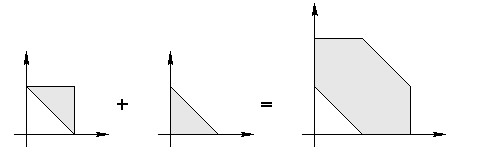
\includegraphics{task1a.jpg}

We study a reverse operation to the Minkowski sum. For a given polygon P, we are looking for two polygons A and B such that: 
\begin{itemize}
\item $P$ is the Minkowski sum of $A$ and $B$,
\item $A$ has from $2$ to $4$ different vertices, i.e. it is a segment (2 vertices), a triangle (3 vertices) or a quadrilateral (4 vertices),
\item $A$ should have as many vertices, as possible, i.e.:
\begin {itemize}
\item $A$ should be a quadrilateral, if possible,
\item if $A$ cannot be a quadrilateral, it should be a triangle, if possible,
\item otherwise it should be a segment.
\end{itemize}
\end{itemize}


Clearly, neither $A$ nor $B$ can be equal to $P$ because then the other summand would have to be a point, which is not a valid polygon. 

You are given a set of input files, each containing a description of a polygon P. For each input file you should find the polygons $A$ and $B$, as required above, and create an output file containing descriptions of $A$ and $B$. For the given input files such polygons A and B can always be found. If there are many correct results, you should find and output one of them. You should not submit any programs, just the output files. 
